\documentclass[11pt,a4paper]{article}

% ----- Encoding & fonts (Calibri-like sans-serif look) -----
\usepackage[utf8]{inputenc}
\usepackage[T1]{fontenc}
\usepackage{helvet}
\renewcommand{\familydefault}{\sfdefault}

% Math + formatting
\usepackage{amsmath,amssymb}
\usepackage{enumitem}
\usepackage{setspace}
\usepackage{array}

% Tables
\usepackage{tabularx}

% Figures + drawing
\usepackage{graphicx}
\usepackage{float}
\usepackage{tikz}

% Code listings
\usepackage{listings}
\usepackage{xcolor}

% Links
% ----- Layout -----
\usepackage[margin=1in]{geometry}
\usepackage{array}
\usepackage{tabularx}
\usepackage{enumitem}
\usepackage{graphicx}
\usepackage{float}
\usepackage{xcolor}
\usepackage{parskip}
\usepackage[hidelinks]{hyperref}
\usepackage{amsmath,amssymb}
\usepackage{tikz}
\usetikzlibrary{positioning,arrows.meta,fit,calc,shapes.geometric}
\usepackage{listings}
\usepackage{xcolor}
% ----- Helpers -----
% A blank-cell strut that gives every status-table row a fillable height.
\newcommand{\fillrow}{\rule[-0.9em]{0pt}{2.4em}}
% A short underline for fill-in fields (name / ID).
\newcommand{\fillin}[1]{\underline{\hspace{#1}}}
% An answer area: a label followed by reserved vertical space.
\newcommand{\answerspace}[1]{%
  \par\vspace{1mm}\noindent\textit{Answer / images:}\par\vspace{#1}%
}
\newcommand{\templatetitle}[1]{%
  \begin{center}
    {\fontsize{22pt}{26pt}\selectfont\textbf{\underline{#1}}}
  \end{center}
}

\newcommand{\templatesection}[1]{%
  \vspace{4pt}
  {\fontsize{14pt}{18pt}\selectfont\textbf{\underline{#1}}}
  \vspace{2pt}
}

\newcommand{\templatesubsection}[1]{%
  \textbf{\underline{#1}}
}
\definecolor{codebg}{rgb}{0.96,0.96,0.94}

\setlength{\parindent}{0pt}
\lstset{
    backgroundcolor=\color{codebg},
    basicstyle=\ttfamily\footnotesize,
    keywordstyle=\color{magenta},
    numberstyle=\tiny\color{gray},
    numbers=left,
    numbersep=8pt,
    frame=none,
    breaklines=true,
    showstringspaces=false,
    tabsize=4,
    xleftmargin=1.5em,
    aboveskip=10pt,
    belowskip=10pt,
}
\begin{document}

% ======================================================================
%  PART 0 - Title block (exact replica of the .docx template)
% ======================================================================
\begin{center}
  {\fontsize{22}{26}\selectfont \textbf{FPGA experiment report}}
\end{center}

\vspace{0.5em}
Task: FPGA 4

\vspace{1em}
Student 1\hspace{1.5em}name: \underline{Mahmood Stitia}\hspace{2em}ID: \underline{214032682}

Student 2:\hspace{1.5em}name: \underline{Saleh Khalil}\hspace{3.2em}ID: \underline{213310485}

\vspace{1.5em}

% ======================================================================
%  PART 1 - Status update
% ======================================================================
{\fontsize{14}{17}\selectfont \textbf{Part 1 - Status update}}

\vspace{0.5em}
Fill in the following table according to your progress at the time of the submission.
Each row should refer to one of the modules together with its simulation.

The status column should be filled with one of the following:
\begin{itemize}[noitemsep,topsep=2pt]
  \item Done - If both are written and simulation passed.
  \item Partially done - If you started writing the module and simulation but it's not working properly.
  \item Not started - If you didn't get to that part of the task.
\end{itemize}

When the status is partially done, please use the notes/comments column to explain in a few more words what is the status of the module and what is the status of the simulation.

\vspace{0.5em}
Fill here:

\vspace{0.5em}
\begin{tabularx}{\textwidth}{|p{3.8cm}|p{3cm}|X|}
\hline
Module name/Step & status & notes/comments \\ \hline
\fillrow Control                       & Done & TB Passed \\ \hline
\fillrow Debouncer                     & Done & \\ \hline
\fillrow Stopwatch                     & Done & \\ \hline
\fillrow Elaborated Design             & Done & \\ \hline
\fillrow Synthesis                     & Done & \\ \hline
\fillrow Setting up constraints        & Done & \\ \hline
\fillrow Implementing the design       & Done & \\ \hline
\fillrow FPGA programming and debugging & Done & \\ \hline
\end{tabularx}

\vspace{1.5em}
\textbf{Issues:}

In this section please describe the current issues you are facing.
\begin{itemize}[noitemsep,topsep=2pt]
  \item Per each module and simulation, if you receive any errors at the time of submission, please describe which errors and what they mean.
\end{itemize}

Fill here:
\begin{itemize}[topsep=2pt]
  \item Control:
  \item Debouncer:
  \item Stopwatch:
  \item Elaborated Design:
  \item Synthesis:
  \item Setting up constraints:
  \item Implementing the design:
  \item FPGA programming and debugging:
\end{itemize}

\vspace{1.5em}

% ======================================================================
%  PART 2 - Simulations and answers
% ======================================================================
{\fontsize{14}{17}\selectfont \textbf{Part 2 - Simulations and answers}}

\vspace{0.5em}
In this section, please add the images for each simulation as described in the report. Remember to use annotations and explain in your own words what is shown in each simulation.

In some of the tasks in the report, there are also questions that you should answer here.

Make sure to include images of all simulations running at the time of submission, even if they are not correct.

\vspace{0.5em}
Fill here:

\begin{itemize}[topsep=4pt,itemsep=8pt,leftmargin=1.5em]
\newpage
% ------------------------------------------------------------------
\item \textbf{Control:}

\textbf{2c. Test-bench.} The test-bench exhaustively drives the FSM from each of the three reachable states (\texttt{IDLE}, \texttt{COUNTING}, \texttt{PAUSED}) and applies every possible combination of \texttt{\{reset,trig,split\}} (\texttt{cii} = $0\ldots7$).

\begin{figure}[H]
    \centering
    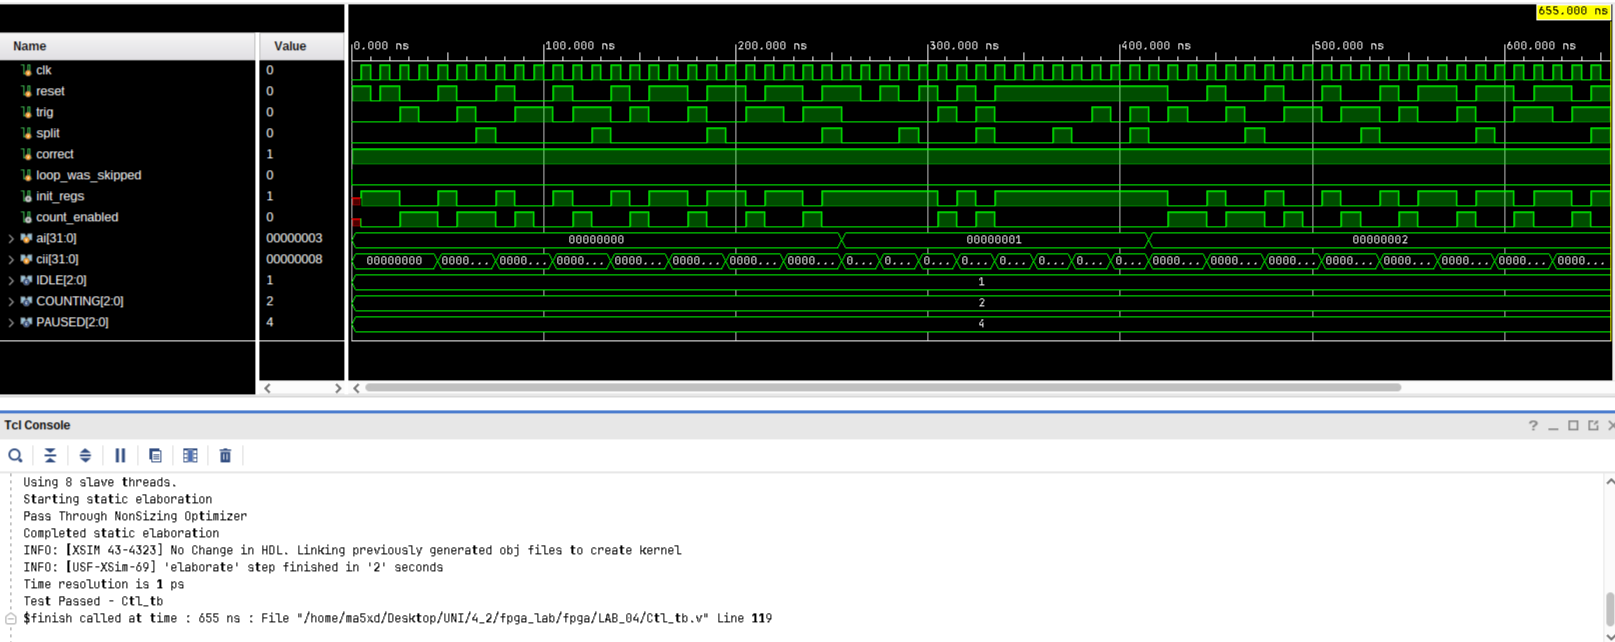
\includegraphics[width=\linewidth]{control_withTEST_passed.png}
    \caption{Annotated waveform of \texttt{Ctl\_tb}. The outer counter \texttt{ai} sweeps the three starting states (IDLE $= 0$, COUNTING $= 1$, PAUSED $= 2$) and the inner counter \texttt{cii} sweeps the 8 input combinations of \texttt{\{reset,trig,split\}}. The \texttt{correct} signal stays high for the whole simulation, and the TCL console at the bottom shows \texttt{Test Passed - Ctl\_tb} and Corrent was high all the time}
\end{figure}
%what the fuck are you doing ?
\begin{figure}[H]
    \centering
    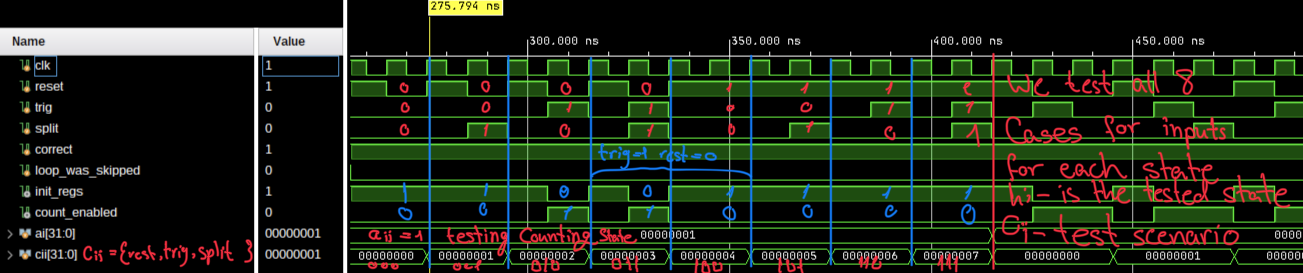
\includegraphics[width=\linewidth]{control_extra.png}
     \caption{Zoomed view inside the \texttt{ai = 1} (COUNTING) block. After the short preamble (one \texttt{reset} pulse, then one \texttt{trig} pulse to leave IDLE), the FSM is in COUNTING and \texttt{count\_enabled} is high. Each subsequent \texttt{cii} value tests one of the COUNTING transitions in Figure 1: a \texttt{trig} pulse drops \texttt{count\_enabled} (move to PAUSED) and a later \texttt{reset} forces \texttt{init\_regs} high (return to IDLE).}
\end{figure}

\textbf{2d.ii Mealy vs.\ Moore.} The assignment draws the FSM in Mealy form (each arrow shows \emph{both} inputs and outputs). However, all transitions \emph{leaving the same state} carry the \emph{same output}:
\begin{itemize}[noitemsep,topsep=2pt]
    \item every arrow leaving \texttt{IDLE} outputs \texttt{init\_regs,count\_enabled = 10},
    \item every arrow leaving \texttt{COUNTING} outputs \texttt{01},
    \item every arrow leaving \texttt{PAUSED} outputs \texttt{00}.
\end{itemize}
The output therefore depends only on the current state, so this FSM is in fact a \textbf{Moore} FSM. This is exactly how the output is written in \texttt{Ctl.v}:
\[
\texttt{init\_regs} = (\texttt{state} == \texttt{IDLE}), \qquad
\texttt{count\_enabled} = (\texttt{state} == \texttt{COUNTING}).
\]

% ------------------------------------------------------------------
% \newpage
\vspace{2cm}
\item \textbf{Debouncer:}

\textbf{3c. High vs.\ low \texttt{COUNTER\_BITS} -- the tradeoff.}

The hysteresis counter must climb from $0$ to $2^{\texttt{COUNTER\_BITS}-1}$ for the MSB to flip and emit a single-cycle pulse. With a $100\,\text{MHz}$ clock the debounce window is therefore
\[
T_{\text{debounce}} \approx \frac{2^{\texttt{COUNTER\_BITS}-1}}{f_{\text{clk}}}.
\]
For the value we use in the top module (\texttt{COUNTER\_BITS}\,$= 20$), $T_{\text{debounce}} \approx 2^{19}/10^{8}\,\text{s} \approx 5.24\,\text{ms}$, comfortably above the typical $1$--$2\,\text{ms}$ contact bounce of a tactile button.


The \texttt{COUNTER\_BITS} parameter determines the duration of the debounce interval. Increasing its value enlarges the counter, which improves immunity to noise and contact bouncing but also introduces longer latency before the system responds to a button press. Conversely, reducing this value shortens response time but increases the likelihood of false triggering caused by unstable or noisy input signals.\\\\This tradeoff is directly analogous to the low-pass-filter-based debouncing approach from earlier experiments. A lower cutoff frequency averages the input over a longer time, suppressing bouncing at the cost of increased delay, while a higher cutoff frequency allows faster response with reduced noise suppression. Similarly, a larger counter value requires longer input stability, whereas a smaller counter value reacts faster but is more sensitive to noise.
\newpage
% ------------------------------------------------------------------
\newpage
\item \textbf{Stopwatch:}

\textbf{4a. Block diagram and connectivity.}

\begin{figure}[h]
\centering
\includegraphics[width=\textwidth]{FPGA_stopwatch-Page-2.png}
\caption{block diagram for the Stopwatch module}
\label{fig:your_label}

\vspace{1em} % Add some vertical space between the image and the list

\begin{tabular}{ll}
\textbf{Input Signals:} & \\
clk & Clock input \\
btnC &  Center Button input \\
btnU &  Upper Button input \\
btnR &  Right Button input \\
btnL &  Left Button input \\
\\
\textbf{Output Signals:} & \\
seg[6:0] & 7-segment display control \\
an[3:0] & Anode control for multiplexed display \\
dp & Decimal point control \\
led\_left[2:0] & Left set of LEDs \\
led\_right[2:0] & Right set of LEDs \\
\end{tabular}
\end{figure}
% ------------------------------------------------------------------
\newpage
\item \textbf{Elaborated Design:}

\textbf{5b. Elaborated-design schematic.}

\begin{figure}[H]
    \centering
    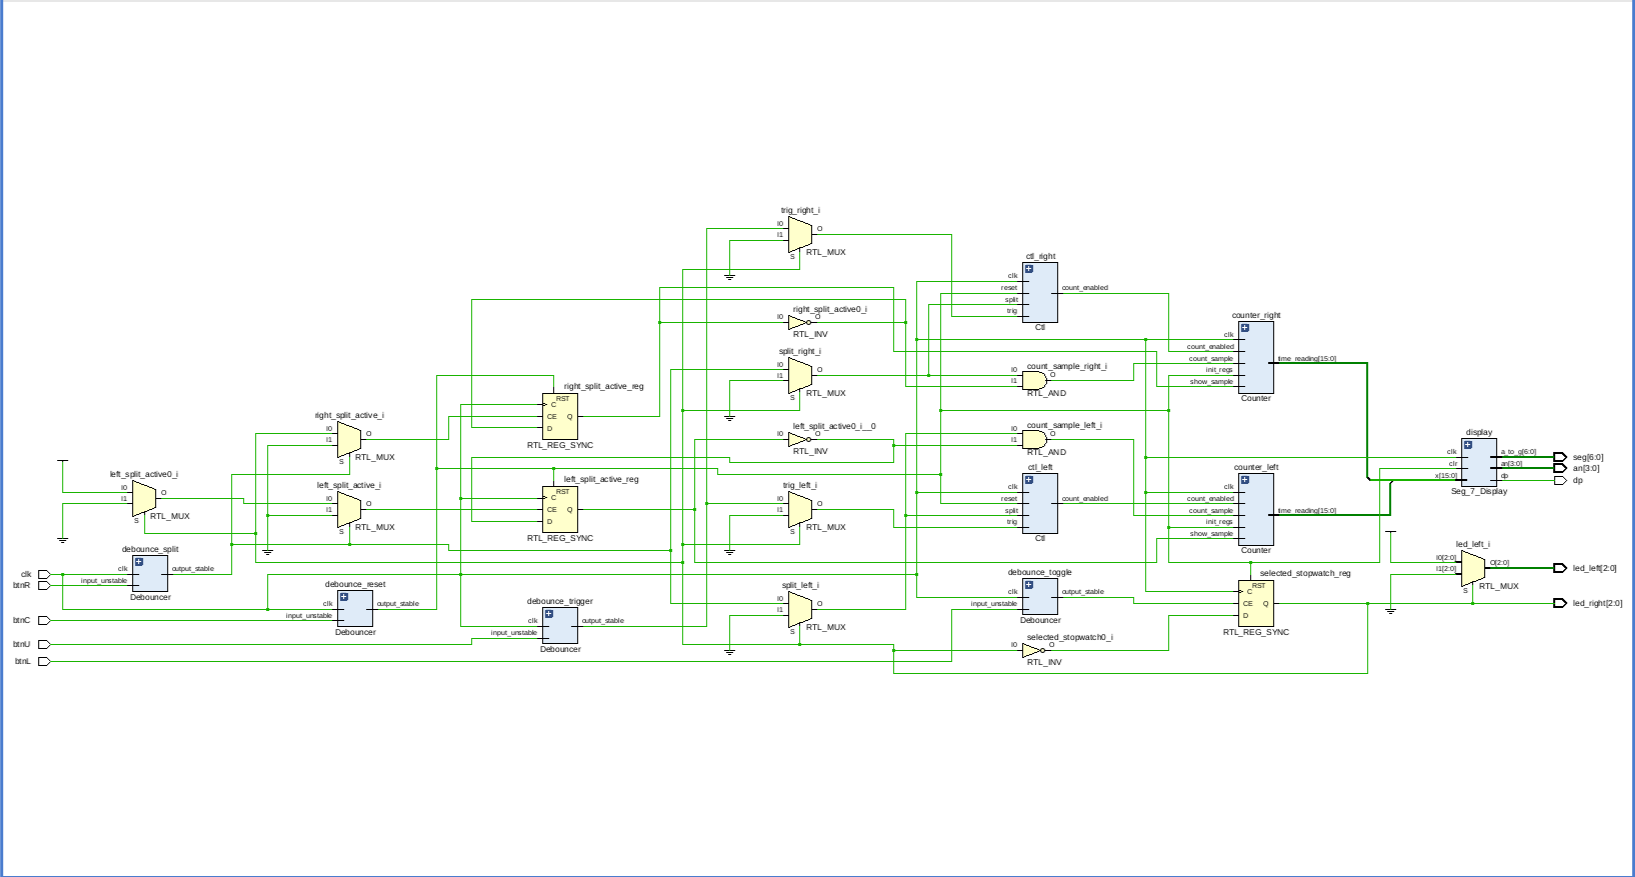
\includegraphics[width=\linewidth]{5a_rtl_sch.png}
    \caption{RTL-elaborated schematic of \texttt{Stopwatch}. All four \texttt{Debouncer} instances, the two \texttt{Ctl} blocks, the two \texttt{Counter} blocks and the shared \texttt{Seg\_7\_Display} appear as hierarchical boxes. The orange \texttt{RTL\_MUX} gates implement the input routing (trig / split go only to the selected side), \texttt{RTL\_AND} gates produce the \texttt{count\_sample} pulses (\texttt{split \& \textasciitilde split\_active}), and the synchronous \texttt{RTL\_REG\_SYNC} elements are the \texttt{selected\_stopwatch}, \texttt{left\_split\_active} and \texttt{right\_split\_active} registers. All top-level ports (\texttt{btnC}, \texttt{btnU}, \texttt{btnR}, \texttt{btnL}, \texttt{clk} on the left and \texttt{seg[6:0]}, \texttt{an[3:0]}, \texttt{dp}, \texttt{led\_left[2:0]}, \texttt{led\_right[2:0]} on the right) are present.}
\end{figure}

% ------------------------------------------------------------------
\newpage
\item \textbf{Synthesis:}

\textbf{6c.i Synthesized schematic.}

\begin{figure}[H]
    \centering
    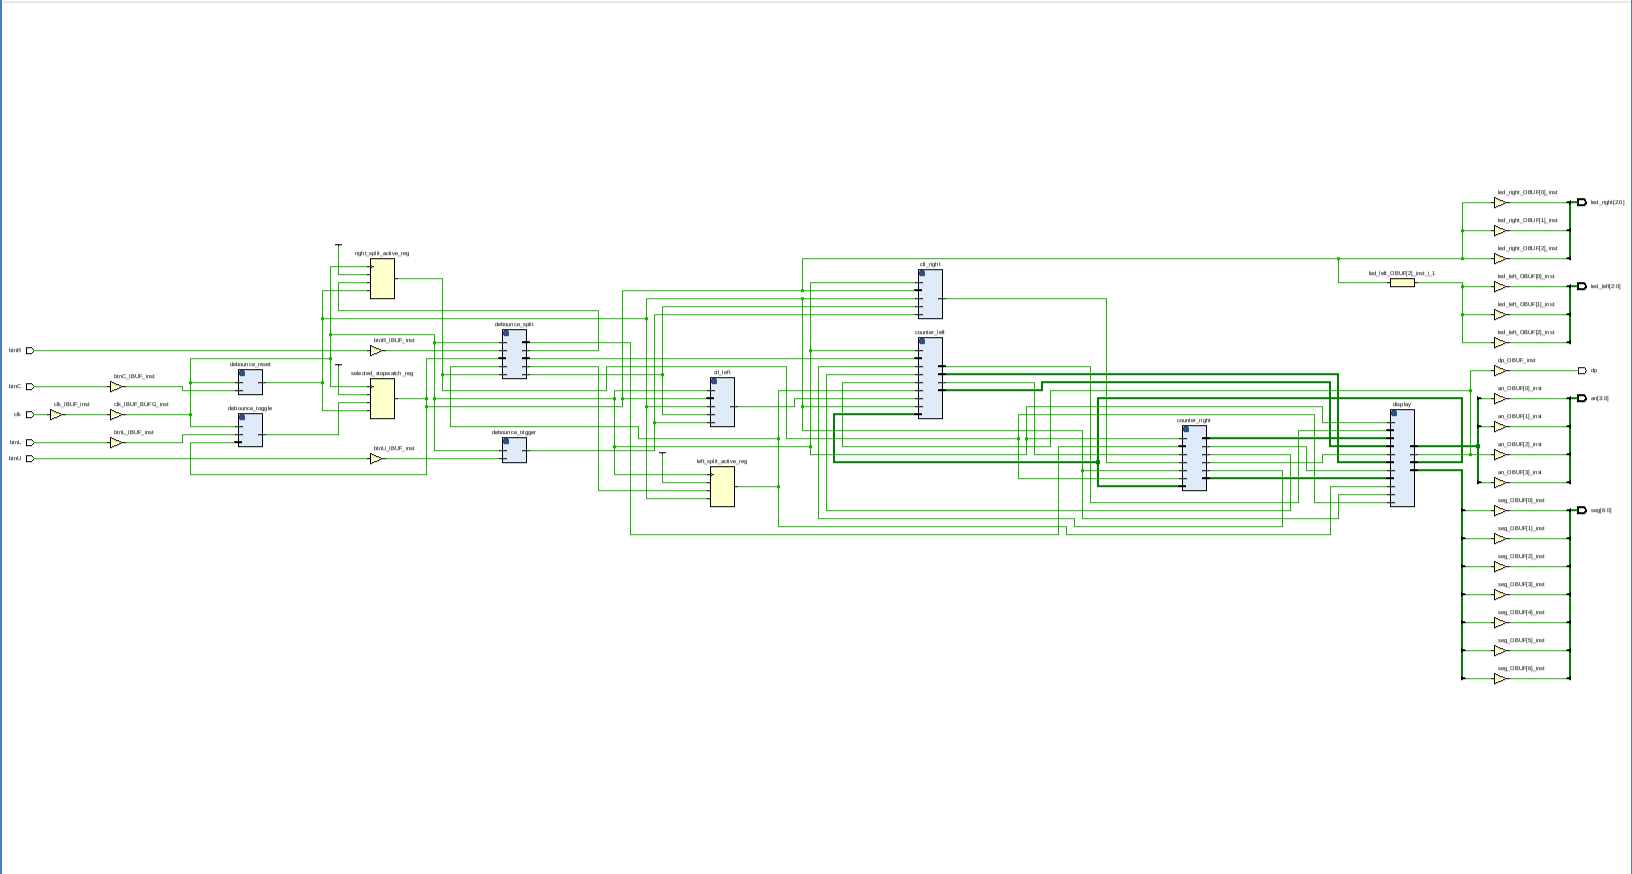
\includegraphics[width=\linewidth]{6c_synth_sch.png}
    \caption{Post-synthesis schematic of \texttt{Stopwatch}. The hierarchical boxes are still recognisable, but every external signal now passes through an \texttt{IBUF} / \texttt{OBUF} I/O buffer, the clock goes through a \texttt{BUFG} global buffer, and the combinational logic inside each block has been mapped onto LUTs and FDRE/FDSE flip-flops. The \texttt{led\_left} / \texttt{led\_right} OBUFs on the right show that synthesis recognised that the three LEDs of each side share the same drive signal (\texttt{selected\_stopwatch} or its inverse).}
\end{figure}

\textbf{6c.ii Differences between elaborated and synthesized.}   In the elaborated design, we see the logical/behavioral structure as written in Verilog---high-level modules, generic RTL primitives (RTL\_MUX, RTL\_REG, RTL\_AND), and abstract signal buses. After synthesis, Vivado maps the design onto actual FPGA primitives: LUTs (Look-Up Tables), FDREs/FDSEs (flip-flops with reset/set and enable), IBUFs/OBUFs (I/O buffers), and a BUFG (global clock buffer). The synthesizer also performs optimizations such as merging logic, removing unused paths, and flattening hierarchies where beneficial.
\end{itemize}

% ------------------------------------------------------------------
\newpage
\textbf{Implementing the design:}

\textbf{8c.i Timing summary.}

\begin{figure}[H]
    \centering
    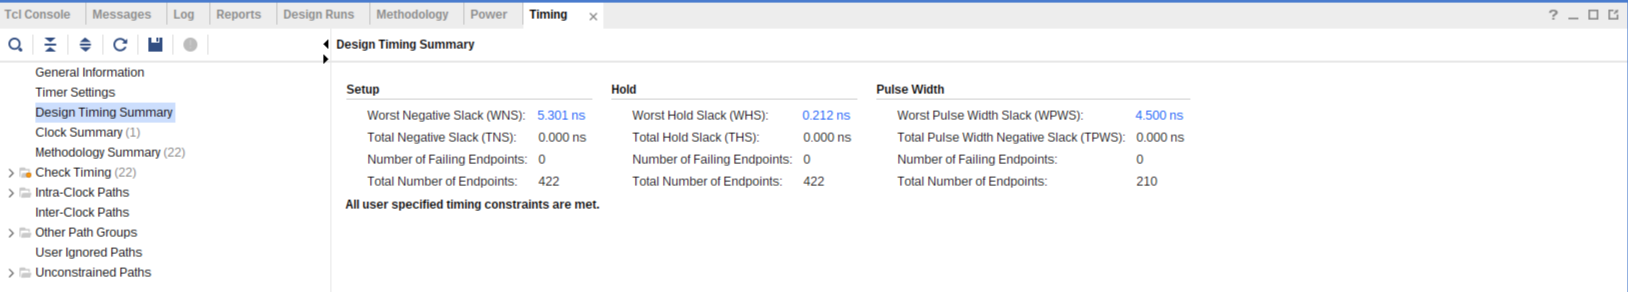
\includegraphics[width=\linewidth]{timing_summary.png}
    \caption{Design Timing Summary after implementation. All user-specified timing constraints are met: the Setup, Hold and Pulse-Width slacks are all positive, with zero failing endpoints in every category.}
\end{figure}

The timing summary reports:
\begin{itemize}[noitemsep,topsep=2pt]
    \item \textbf{Setup:} Worst Negative Slack (WNS) $= 5.301\,\text{ns}$ -- positive $\Rightarrow$ constraint met.
    \item \textbf{Hold:} Worst Hold Slack (WHS) $= 0.212\,\text{ns}$ -- positive $\Rightarrow$ constraint met.
    \item \textbf{Pulse Width:} Worst Pulse-Width Slack (WPWS) $= 4.500\,\text{ns}$ -- positive $\Rightarrow$ constraint met.
    \item Number of Failing Endpoints: $0$ in every category (out of $422$ setup/hold endpoints and $210$ pulse-width endpoints).
\end{itemize}

\textbf{8c.ii Critical setup path length.}

Working from the WNS first, the setup slack is the gap between the clock period and the longest data path:
\begin{align*}
\text{slack}_{\text{setup}} &= T_{\text{clk}} - T_{\text{critical}} - T_{\text{uncertainty}} \\
5.301\,\text{ns} &\approx 10\,\text{ns} - T_{\text{critical}} \\
T_{\text{critical}} &\approx 4.699\,\text{ns}.
\end{align*}

Vivado's Intra-Clock Paths report confirms this directly:

\begin{figure}[H]
    \centering
    
\includegraphics[width=\linewidth]{critical_path.png}
    \caption{Intra-Clock Paths -- Setup. The critical setup path (Path 1) runs from \texttt{counter\_left/clk\_cnt\_reg[19]/C} to \texttt{counter\_left/on\ldots seconds\_reg[0]/D}, with a total datapath delay of $4.743\,\text{ns}$ ($1.212\,\text{ns}$ logic + $3.531\,\text{ns}$ net), $4$ logic levels and a slack of $5.301\,\text{ns}$ against the $10\,\text{ns}$ requirement.}
\end{figure}

The reported total path length is therefore $\boxed{T_{\text{critical}} = 4.743\,\text{ns}}$. The very small difference from the $4.699\,\text{ns}$ derived from the slack is the clock uncertainty/jitter term that Vivado subtracts separately. For completeness, the worst hold path is shown below:

\begin{figure}[H]
    \centering
    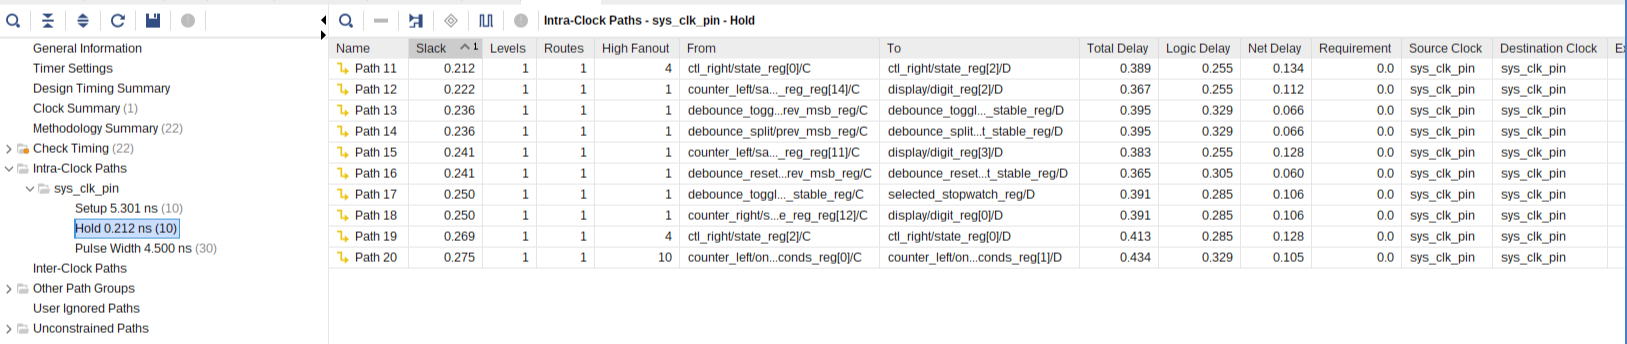
\includegraphics[width=\linewidth]{critical_path_hold.png}
    \caption{Intra-Clock Paths -- Hold. The worst hold path (Path 11) runs inside \texttt{ctl\_right} between two adjacent state-register bits, with a total delay of $0.389\,\text{ns}$ and a positive slack of $0.212\,\text{ns}$, confirming that no flip-flop violates its hold time.}
\end{figure}

% ------------------------------------------------------------------
\newpage
\textbf{FPGA programming and debugging:}

\textbf{9a-b.} On hardware the two stopwatches behave as specified:
\begin{itemize}[noitemsep,topsep=2pt]
    \item \texttt{btnL} toggles the selection between the left and right stopwatches; the \texttt{led\_left} / \texttt{led\_right} bars indicate which side is active.
    \item \texttt{btnU} (trig) starts and pauses \emph{only} the currently selected stopwatch; the other side keeps running unaffected.
    \item \texttt{btnR} (split) freezes / unfreezes the displayed value of the currently selected side without stopping the underlying counter.
    \item \texttt{btnC} (reset) zeroes both stopwatches and brings the selection back to the left side.
\end{itemize}

\textbf{9c. Post-implementation project summary.} After verifying the design on hardware, the debug core was removed and the design was re-implemented to obtain the final post-implementation reports:

\begin{figure}[H]
    \centering
    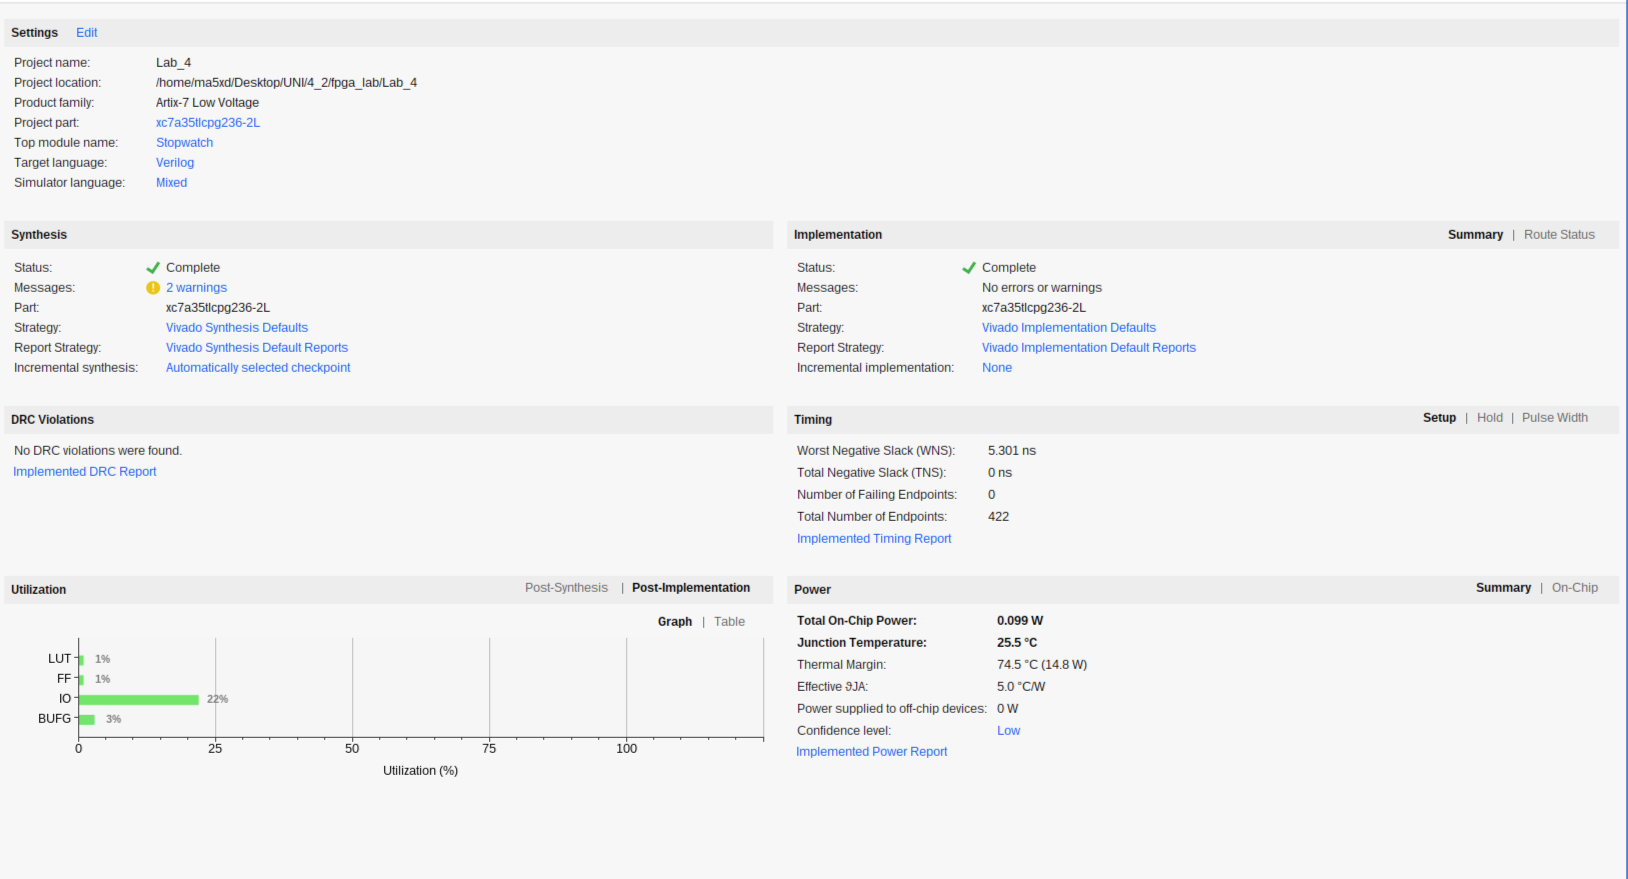
\includegraphics[width=\linewidth]{proj_summary.png}
    \caption{Project Summary after implementation}
\end{figure}

\begin{figure}[H]
    \centering
    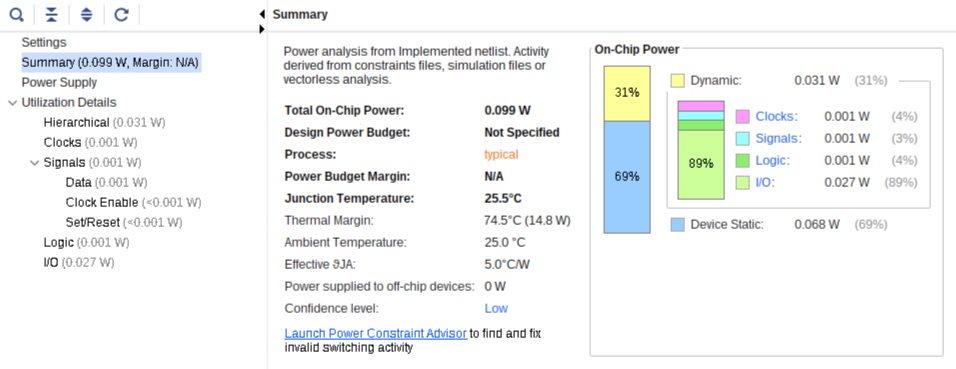
\includegraphics[width=0.85\linewidth]{power_summary.png}
    \caption{Power report. Total on-chip power is $0.099\,\text{W}$, of which $0.031\,\text{W}$ ($31\%$) is dynamic (mostly I/O at $0.027\,\text{W}$) and $0.068\,\text{W}$ ($69\%$) is device static. Junction temperature is $25.5^{\circ}\text{C}$ with a thermal margin of $74.5^{\circ}\text{C}$ ($14.8\,\text{W}$).}
\end{figure}
\newpage

% ======================================================================
%  PART 3 - Verilog source code appendix
% ======================================================================
\templatesection{Appendix -- Verilog Source Code}

\vspace{6pt}


\begin{figure}[H]
    \centering
    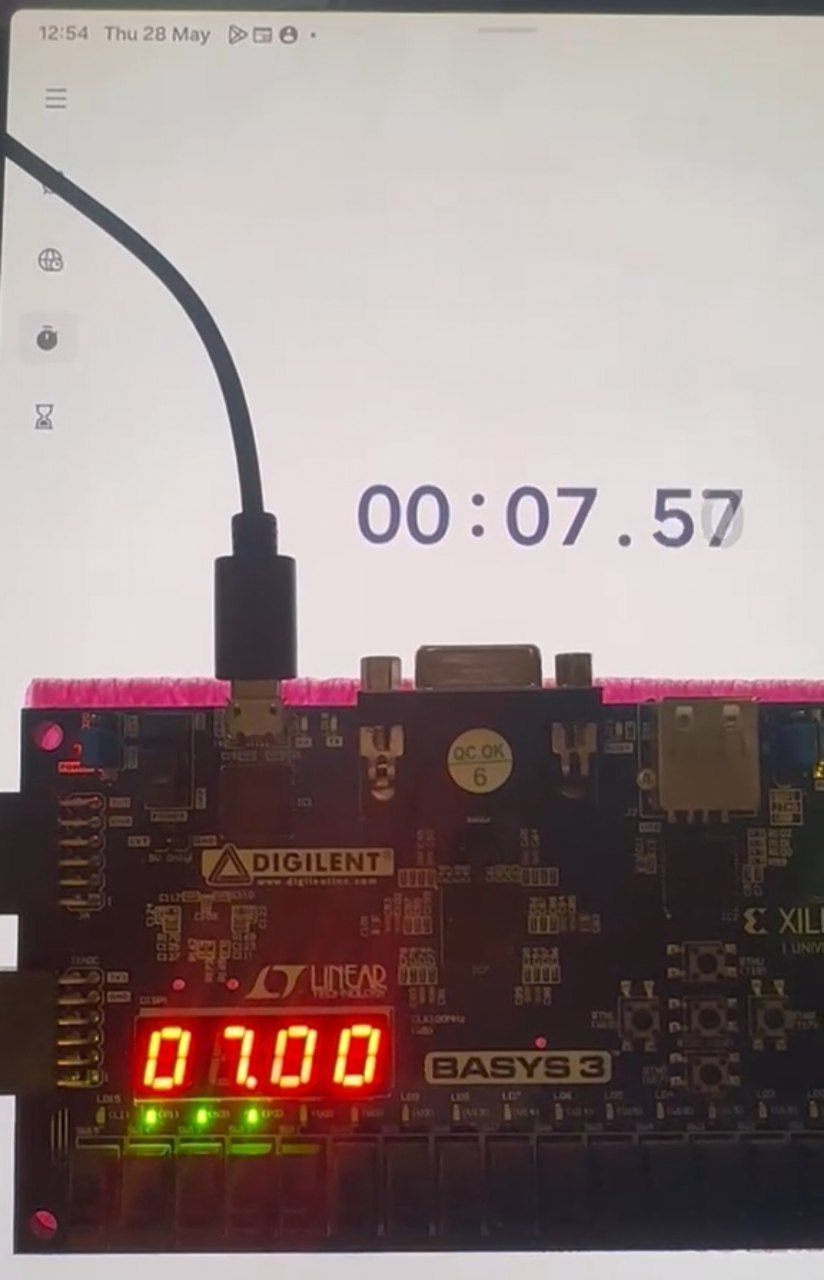
\includegraphics[width=0.75\linewidth]{photo1.jpg}
    \caption{Stopwatch at 07.00 seconds, with the left side selected and split active. The left two digits show the frozen value of the left stopwatch (07), while the right two digits show the live value of the right stopwatch (00).}
\end{figure}

\begin{figure}[H]
    \centering
    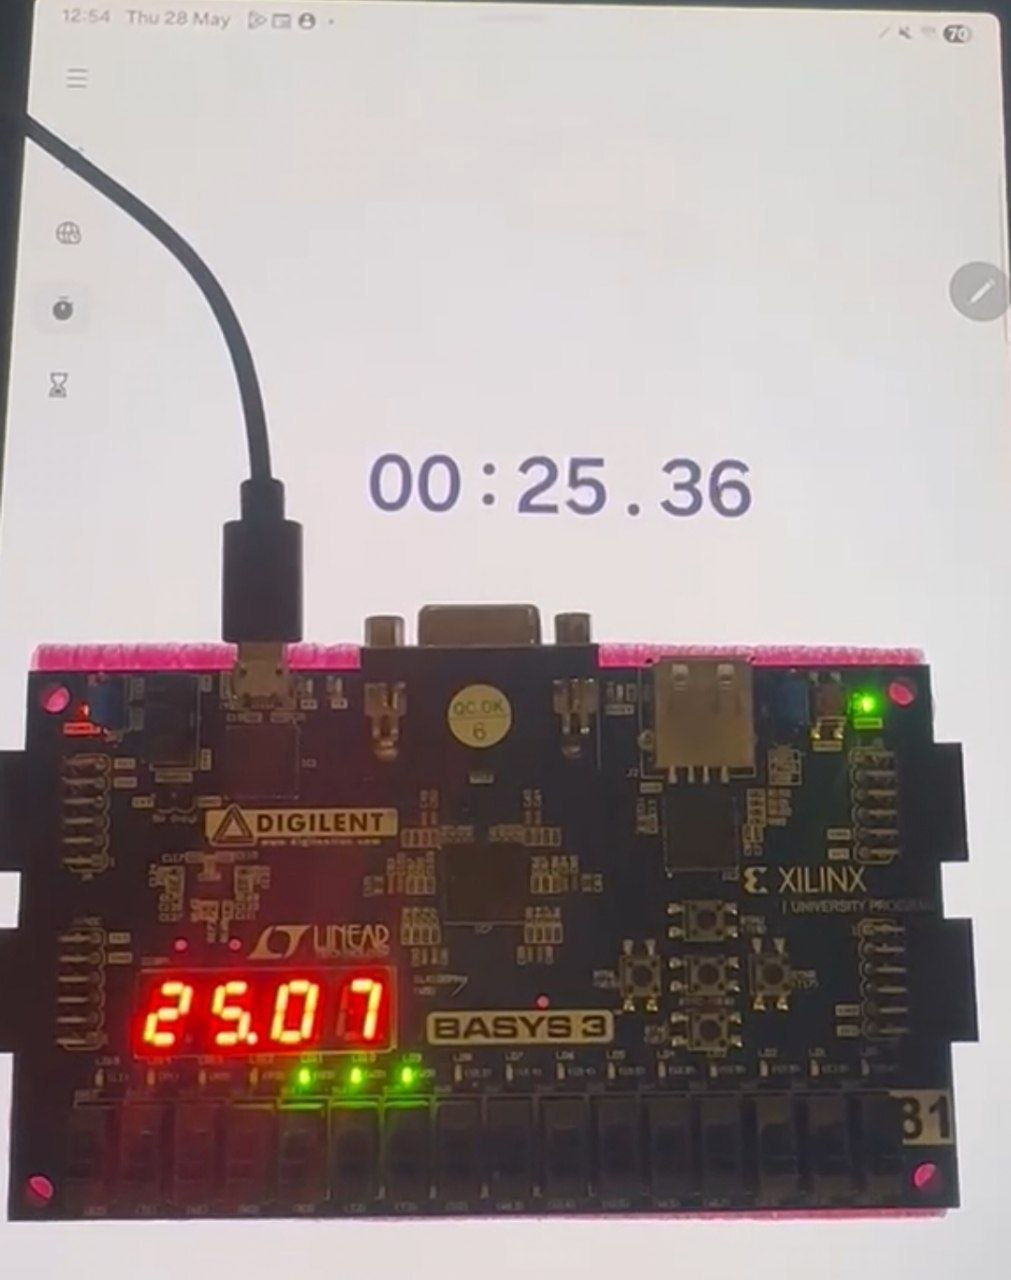
\includegraphics[width=0.75\linewidth]{photo2.jpg}
    \caption{Stopwatch at 25.07 seconds, with the right side selected as the LED indicator shows. The left two digits show the value of the left stopwatch (25), while the right two digits show the value of the right stopwatch (07).}
\end{figure}


\newpage

Ctl.v

\begin{lstlisting}
`timescale 1ns/10ps
module Ctl(clk, reset, trig, split, init_regs, count_enabled);

   input  clk, reset, trig, split;
   output init_regs, count_enabled;

   localparam SIZE = 3;
   localparam IDLE = 3'b001, COUNTING = 3'b010, PAUSED = 3'b100;
   reg [SIZE-1:0] state;

   always @(posedge clk) begin
      if (reset)
         state <= IDLE;
      else begin
         case (state)
            IDLE     : state <= (trig)? COUNTING : IDLE;
            COUNTING : state <= (trig)? PAUSED   : COUNTING;
            PAUSED   : begin
               casez({reset, trig, split})
                  3'b000 : state <= PAUSED;
                  3'b001 : state <= IDLE;
                  3'b01? : state <= COUNTING;
                  3'b1?? : state <= IDLE;
                  default: state <= PAUSED;
               endcase
            end
            default  : state <= IDLE;
         endcase
      end
   end

   assign init_regs     = (state == IDLE);
   assign count_enabled = (state == COUNTING);

endmodule
\end{lstlisting}

\clearpage
Ctl\_tb.v

\begin{lstlisting}
module Ctl_tb();
    reg clk, reset, trig, split, correct, loop_was_skipped;
    wire init_regs, count_enabled;
    integer ai, cii;
    localparam IDLE = 3'b001, COUNTING = 3'b010, PAUSED = 3'b100;
    Ctl uut(.clk(clk), .reset(reset), .trig(trig), .split(split),
            .init_regs(init_regs), .count_enabled(count_enabled));
    initial begin
        correct = 1; loop_was_skipped = 0;
        ai = 0; cii = 0;
        clk = 0; reset = 1; trig = 0; split = 0;
        #10 reset = 0;
        correct = correct & init_regs & ~count_enabled;
        @(posedge clk);
        loop_was_skipped = 1;
        for (ai = 0; ai < 3; ai = ai + 1) begin
            loop_was_skipped = 0;
            for (cii = 0; cii < 8; cii = cii + 1) begin
                reset = 1; #10 reset = 0;
                if (ai != IDLE)   begin trig = 1; #10 trig = 0; end
                if (ai == PAUSED) begin trig = 1; #10 trig = 0; end
                {reset, trig, split} = cii;
                #10
                {reset, trig, split} = 0;
                case (ai)
                    IDLE: casez(cii)
                        3'b00? : correct = correct & init_regs & ~count_enabled & (uut.state == IDLE);
                        3'b1?? : correct = correct & init_regs & ~count_enabled & (uut.state == IDLE);
                        3'b01? : correct = correct & ~init_regs & count_enabled & (uut.state == COUNTING);
                        default: correct = 0;
                    endcase
                    COUNTING: casez(cii)
                        3'b1?? : correct = correct & init_regs & ~count_enabled & (uut.state == IDLE);
                        3'b00? : correct = correct & ~init_regs & count_enabled & (uut.state == COUNTING);
                        3'b01? : correct = correct & ~init_regs & ~count_enabled & (uut.state == PAUSED);
                        default: correct = 0;
                    endcase
                    PAUSED: casez(cii)
                        3'b1?? : correct = correct & init_regs & ~count_enabled & (uut.state == IDLE);
                        3'b01? : correct = correct & ~init_regs & count_enabled & (uut.state == COUNTING);
                        3'b001 : correct = correct & init_regs & ~count_enabled & (uut.state == IDLE);
                        3'b000 : correct = correct & ~init_regs & ~count_enabled & (uut.state == PAUSED);
                        default: correct = 0;
                    endcase
                endcase
            end
        end
        if (correct) $display("Test Passed - %m");
        else         $display("Test Failed - %m");
        $finish;
    end
    always #5 clk = ~clk;
endmodule
\end{lstlisting}
\vspace{2 cm}
Debouncer.v

\begin{lstlisting}
`timescale 1ns/10ps
module Debouncer(clk, input_unstable, output_stable);

   input  clk, input_unstable;
   output reg output_stable;

   parameter COUNTER_BITS = 7;
   reg prev_msb;
   reg [COUNTER_BITS-1:0] counter;

   always @(posedge clk) begin
      if (input_unstable == 1)
         counter <= (counter < {COUNTER_BITS{1'b1}}) ? counter + 1 : counter;
      else
         counter <= (counter > {COUNTER_BITS{1'b0}}) ? counter - 1 : counter;

      prev_msb      <= counter[COUNTER_BITS-1];
      output_stable <= (~prev_msb) & counter[COUNTER_BITS-1];
   end

endmodule
\end{lstlisting}

\clearpage
Stopwatch.v

\begin{lstlisting}
`timescale 1ns/10ps
module Stopwatch(clk, btnC, btnU, btnR, btnL, seg, an, dp, led_left, led_right);

    input              clk, btnC, btnU, btnR, btnL;
    output  wire [6:0] seg;
    output  wire [3:0] an;
    output  wire       dp; 
    output  wire [2:0] led_left;
    output  wire [2:0] led_right;

    wire [15:0] time_reading;
    // button signals
    wire trig, split, reset, toggle;
    // counter signals
    wire trig_right, split_right, init_regs_right, count_enabled_right, count_sample_right, show_sample_right;
    wire trig_left,  split_left,  init_regs_left,  count_enabled_left, count_sample_left, show_sample_left;
    // selected stopwatch
    localparam LEFT = 1'b0, RIGHT = 1'b1;
    reg selected_stopwatch; //left -> 0; right -> 1
    
	// FILL HERE INSTANTIATIONS
    wire [15:0] time_reading_left, time_reading_right;
    // reg right_split_active, left_split_active;

    ///////////////////////////
	// Buttons Stabilization //
    ///////////////////////////
	Debouncer #(.COUNTER_BITS(20)) debounce_reset(
        .clk(clk),
        .input_unstable(btnC),
        .output_stable(reset)
	);
	
	Debouncer #(.COUNTER_BITS(20)) debounce_trigger(
        .clk(clk),
        .input_unstable(btnU),
        .output_stable(trig)
	);
	
	Debouncer #(.COUNTER_BITS(20)) debounce_split(
        .clk(clk),
        .input_unstable(btnR),
        .output_stable(split)
	);
	
	Debouncer #(.COUNTER_BITS(20)) debounce_toggle(
        .clk(clk),
        .input_unstable(btnL),
        .output_stable(toggle)
	);

    ///////////////////////////
    //        Controls       //
    ///////////////////////////
    Ctl ctl_right(
        .clk(clk),
        .reset(reset),
        .trig(trig_right),
        .split(split_right),
        .init_regs(init_regs_right),
        .count_enabled(count_enabled_right)
    );
    Ctl ctl_left(
        .clk(clk),
        .reset(reset),
        .trig(trig_left),
        .split(split_left),
        .init_regs(init_regs_left),
        .count_enabled(count_enabled_left)
    );

    ///////////////////////////
    //   7-Segment Display   //
    ///////////////////////////
    Seg_7_Display display(
        .x(time_reading),
        .clk(clk),
        .clr(reset),
        .a_to_g(seg),
        .an(an),
        .dp(dp) 
    );

    ///////////////////////////
    //        Counters       //
    ///////////////////////////
    Counter counter_right(
        .clk(clk),
        .init_regs(reset | init_regs_right),
        .count_enabled(count_enabled_right),
        .count_sample(count_sample_right),
        .show_sample(show_sample_right),
        .time_reading(time_reading_right)
    );
    Counter counter_left(
        .clk(clk),
        .init_regs(reset | init_regs_left),
        .count_enabled(count_enabled_left),
        .count_sample(count_sample_left),
        .show_sample(show_sample_left),
        .time_reading(time_reading_left)
    );

    ///////////////////////////
    //    Stopwatch Logic    //
    ///////////////////////////

    always @(posedge clk) begin // TOGGLE SELECTED STOPWATCH
        if(reset) begin
            selected_stopwatch <= LEFT;
        end
        else begin
            if(toggle) selected_stopwatch <= ~selected_stopwatch;
        end
    end


    // left stopwatch signals
	assign led_left  = (selected_stopwatch == LEFT)? 3'b111 : 3'b000; // left stopwatch is selected
    assign trig_left   = (selected_stopwatch == LEFT)? trig  : 1'b0;
    assign split_left  = (selected_stopwatch == LEFT)? split : 1'b0;
    assign show_sample_left  = 1'b0;
    assign count_sample_left = 1'b0;

    // right stopwatch signals
    assign led_right = (selected_stopwatch == RIGHT)? 3'b111 : 3'b000; // right stopwatch is selected
    assign trig_right  = (selected_stopwatch == RIGHT)? trig  : 1'b0;
    assign split_right = (selected_stopwatch == RIGHT)? split : 1'b0;
    assign show_sample_right  = 1'b0;
    assign count_sample_right = 1'b0;

    assign time_reading = {time_reading_left[15:8], time_reading_right[15:8]};

endmodule
\end{lstlisting}
\end{document}
